\documentclass[12pt]{article}
 
\usepackage[margin=1in]{geometry} 
\usepackage{amsmath,amsthm,amssymb}
\usepackage{hyperref}
\usepackage{graphicx}
\usepackage{xcolor}
\usepackage[many]{tcolorbox}
\tcbuselibrary{listings}
\usepackage{listings}

\definecolor{lg}{HTML}{f0f0f0}

\newtcblisting{pycode}{
    colback=lg,
    boxrule=0pt,
    arc=0pt,
    outer arc=0pt,
    top=0pt,
    bottom=0pt,
    colframe=white,
    listing only,
    left=15.5pt,
    enhanced,
    listing options={
        basicstyle=\small\ttfamily,
        keywordstyle=\color{blue},
        language=Python,
        showstringspaces=false,
        tabsize=2,
        numbers=left,
        breaklines=true
    },
    overlay={
        \fill[gray!30]
        ([xshift=-3pt]frame.south west)
        rectangle
        ([xshift=11.5pt]frame.north west);
    }
}

\lstset{
    language=Python,
    basicstyle=\small\ttfamily,
}

 
\begin{document}
 
\title{Exercise 1}
\author{Cristian Manuel Abrante Dorta - 888248\\
ELEC-E8125 - Reinforcement Learning}

\maketitle
\section{Task 1}
\label{sec:task-1}

\subsection{Question 1.1}
\label{sec:question-1.1}
\textbf {
    Can the same model, trained to balance for 200 timesteps, also balance the pole for 500 timesteps? Briefily justify your answers.
}\\

For answering this question, first of all the model had to be trained during 500 episodes with a maximum 200 time steps per episode. After the agent is trained with those parameters a plot was generated in order to know the performance of the agent over the episodes:

\begin{figure}[ht]
    \centering
    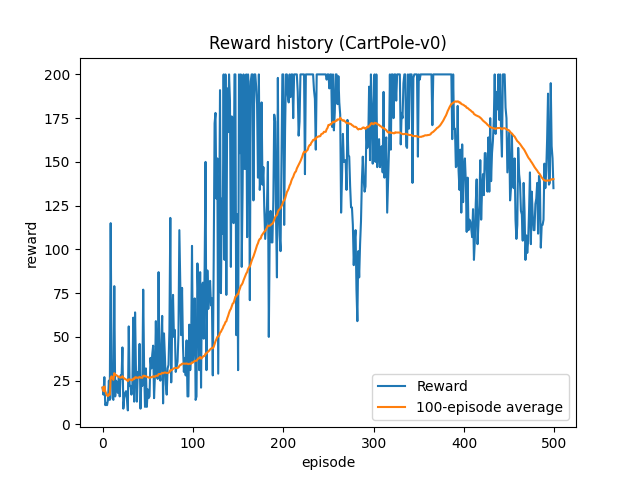
\includegraphics[scale=0.5]{exercise-1/report/img/task-1-training-200.png}
    \caption{Training result with 500 episodes and 200 max time steps per episode.}
    \label{fig:training-200}
\end{figure}

It is important to know that this is not a deterministic process, and that implies that the content of this plot is not the only possible training that the agent could have. But, as we can see in figure \ref{fig:training-200} the cumulative reward (equivalent to the maximum number of time steps that the pole was balanced), is increasing over the training episodes. Obtaining the maximum reward in some intervals between episodes 100 and 400. Also, the average reward have an increasing tendency over all the episodes except from the final 100 episodes. \\

After having trained the model, it was tested with maximum 500 time steps per episode, and the obtained result was:

\begin{center}
    \texttt{Average test reward: 161.644 episode length: 161.644}
\end{center}


\section{Task 2}
To embed code snippets in the report, you can use the \texttt{pycode} environment.

\begin{pycode}
for episode_number in range(train_episodes):
    reward_sum, timesteps = 0, 0
    done = False
    # Reset the environment and observe the initial state
    observation = env.reset()

    # Loop until the episode is over
    while not done:
        # Get action from the agent
        action, action_probabilities = agent.get_action(observation)
        previous_observation = observation

        # Perform the action on the environment, get new state and reward
        observation, reward, done, info = env.step(action)

        # Store action's outcome (so that the agent can improve its policy)
        agent.store_outcome(previous_observation, action_probabilities, action, reward)

        # Draw the frame, if desired
        if render:
            env.render()
\end{pycode}

\section{Question 1}

If you add a figure, you can refer to it using Figure.~\ref*{fig:fig1}.

\begin{figure}[h] 
	\centering  % Remember to centre the figure
    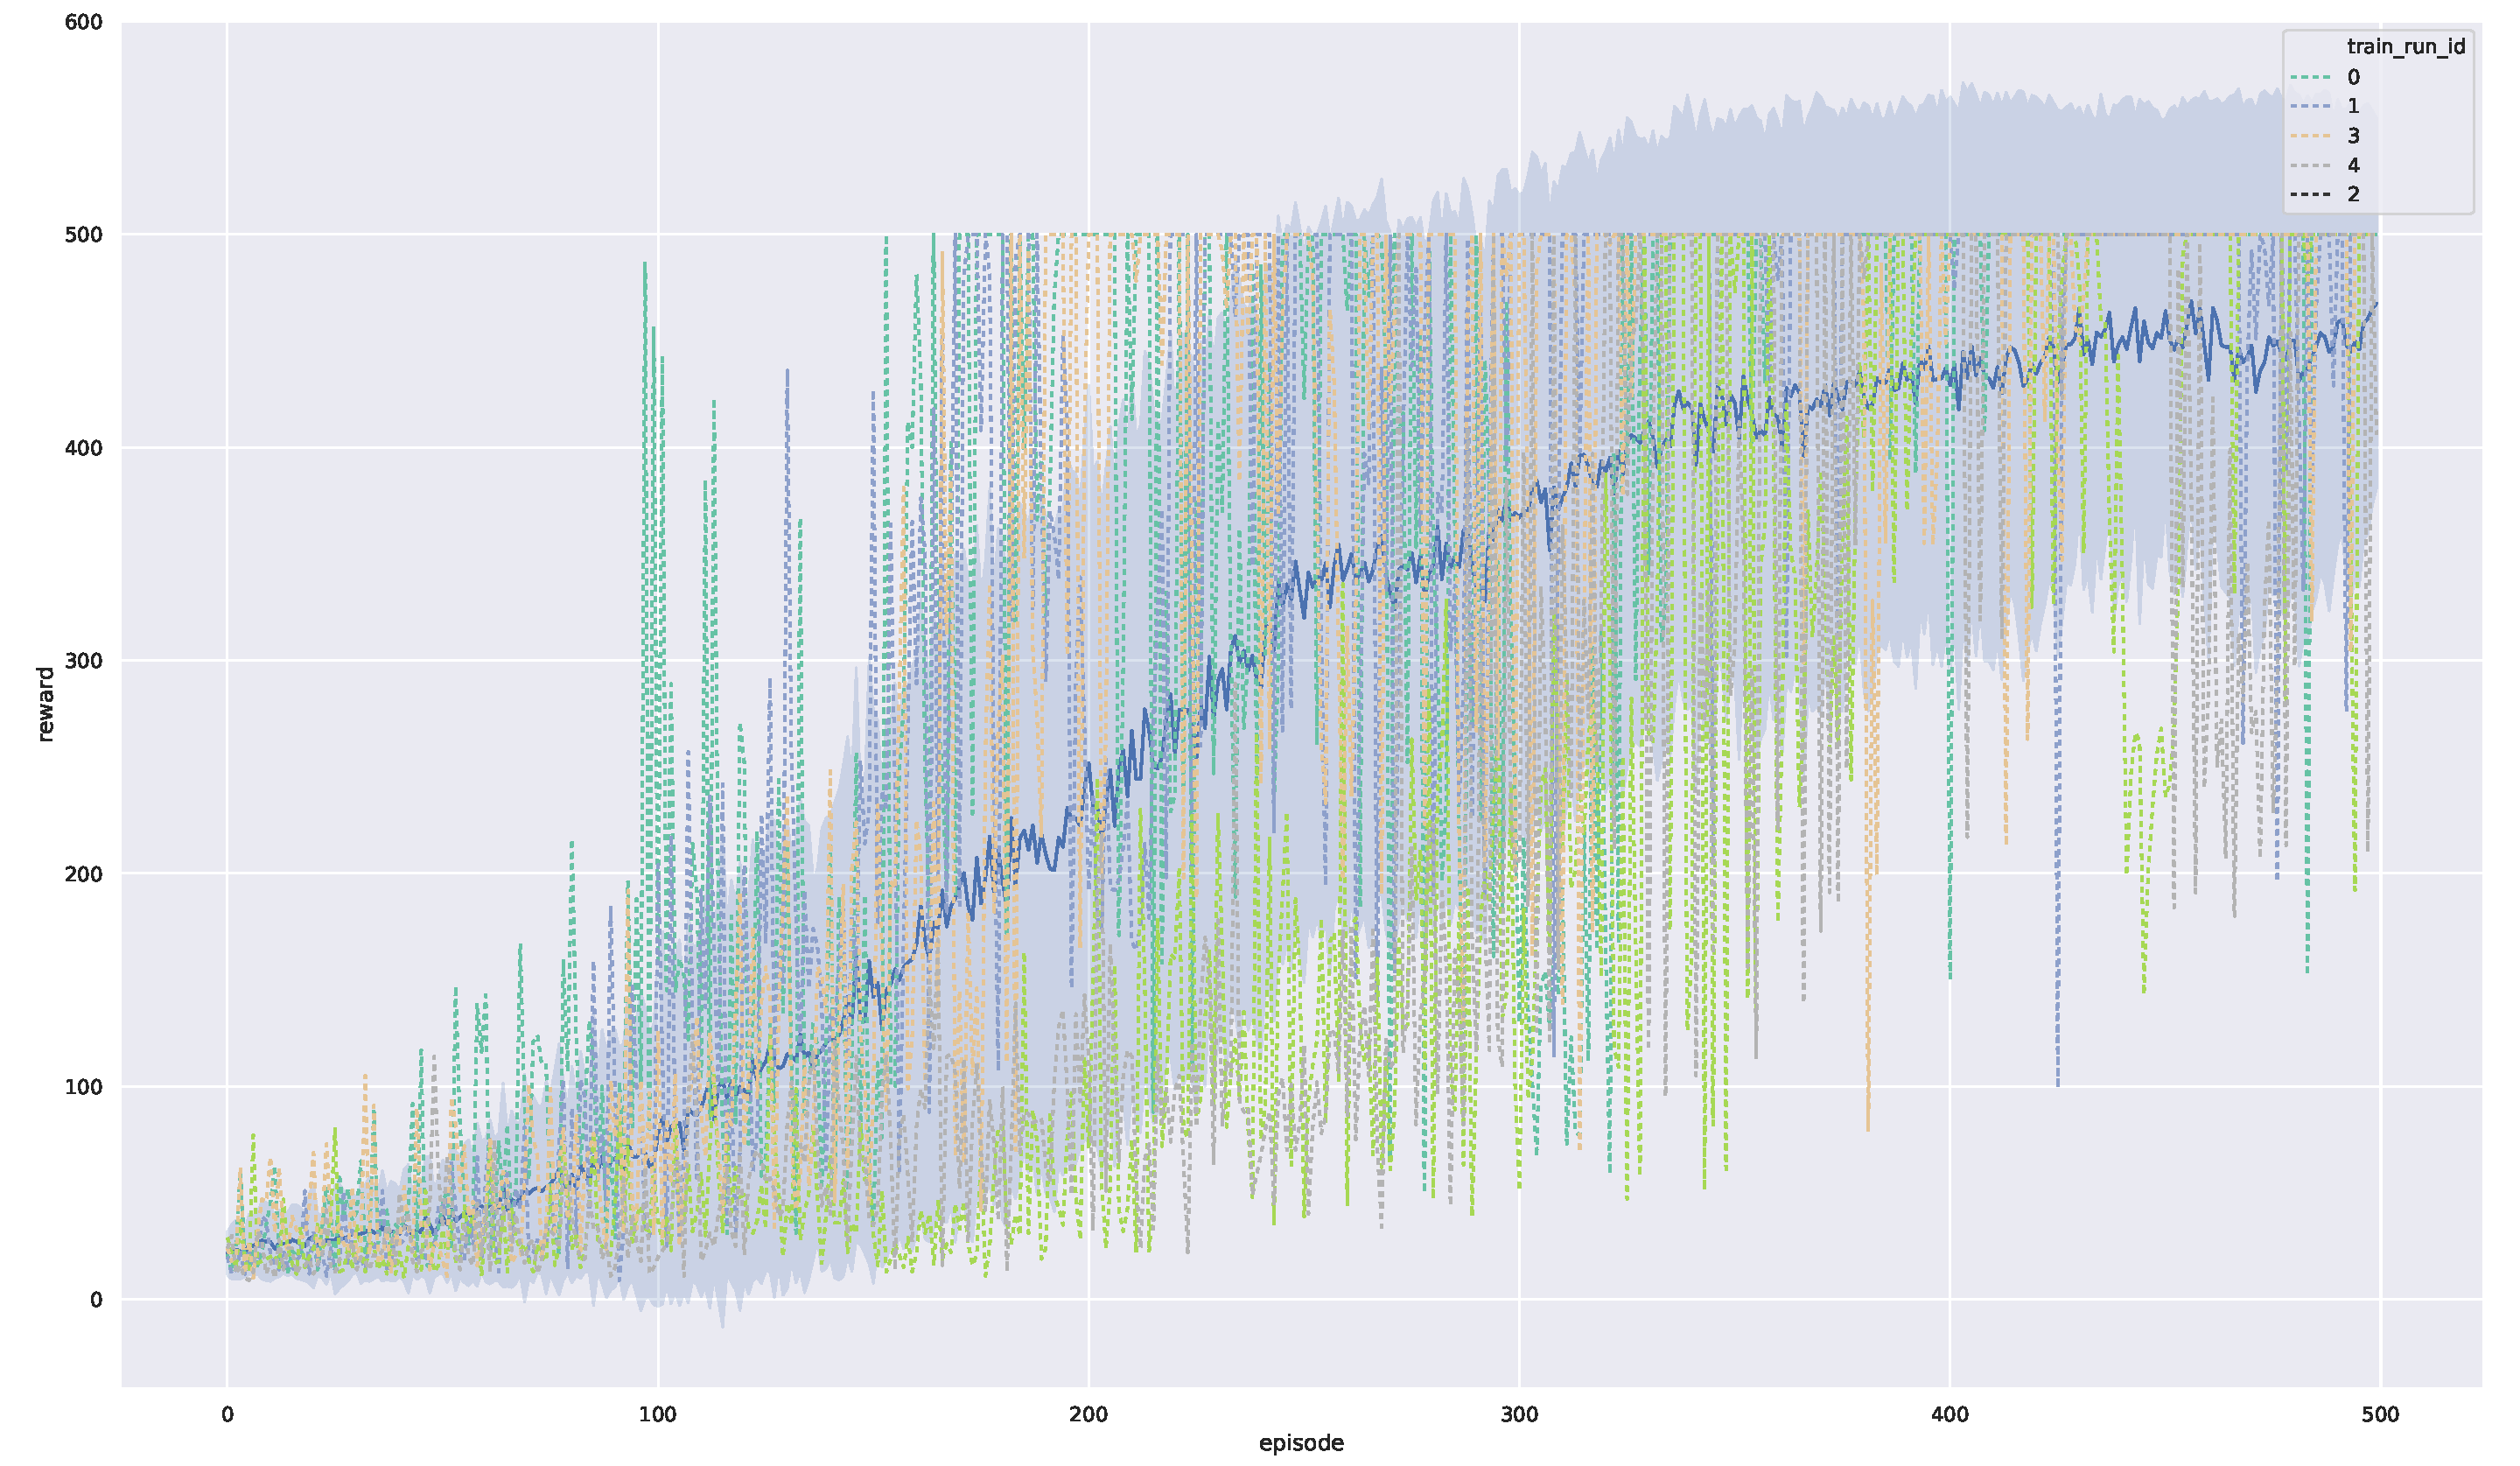
\includegraphics[width=0.9\columnwidth]{img/training.pdf}
	\caption{This is a sample figure.}
	\label{fig:fig1}
\end{figure}

\bibliographystyle{ieeetr}
\bibliography{template}  % Modify template with your bibliography name
\end{document}
